%\subsubsection{Is community growth affected by the number of attractive members?}
Our main goal in this paper is to study evolution of communities residing inside a social network. In particular, we are interested in understanding what parameters affect the growth of a community. In Section \ref{sec: definitions}, 
for the members of a community $\Cc$, we defined the notion of being attractive. In this section, we provide some initial observations connecting the percentage of attractive members of a community to its growth. In Section \ref{sec: regression},  these elementary observations are supported by  regression analysis. 


The growth rate of a community $\Cc$ at snapshot $t$ is defined as
\begin{align}
r_g(t,\Cc) = \frac{|\mathcal{C}_{\mathcal{F}}(t)|}{|\mathcal{C}(t)|},
\end{align}
Let $\bar{r}_g(t)$ denote the average growth rate of the communities under study at snapshot $t$. At each snapshot, we divide the communities into two categories: \emph{growing} and \emph{non-growing}, based on their growth rate at that snapshot.  A community is called growing at snapshot $t$, if its growth rate in that snapshot is larger than the average, i.e., $r_g(t,\Cc) \geq \bar{r}_g(t)$. Otherwise, it is called non-growing.  

For each community $\Cc$, let $p_a(t,\Cc)$ denote the fraction of attractive members of the community at snapshot $t$, i.e.,
\begin{align}
p_a(t,\Cc) = \frac{\sum\limits_{v\in\Cc} a_v}{|\Cc|}.
\end{align}

Fig. \ref{fig: perc_att} shows the fraction of attractive members of growing and non-growing communities for 5 snapshots. 
\begin{figure}
\begin{center}
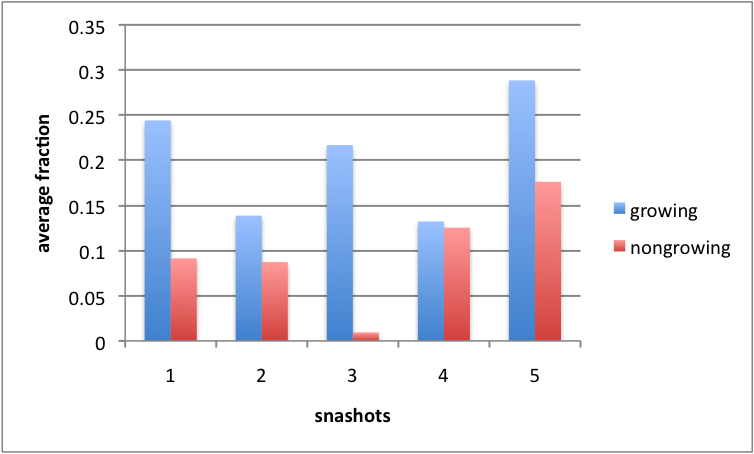
\includegraphics[width=80mm]{../figures/att_growth.png}\caption{Average percentage of attractive members for  growing and non-growing communities in 5 snapshots.}\label{fig: perc_att}
\end{center}
\end{figure}
It can be observed that in all cases the growing communities have on average higher percentage of attractive members. In the next section, we further investigate this observation which demonstrates  some positive correlation between the percentage of  attractive members of a community and its growth.
 



%\begin{figure}
%\begin{center}
%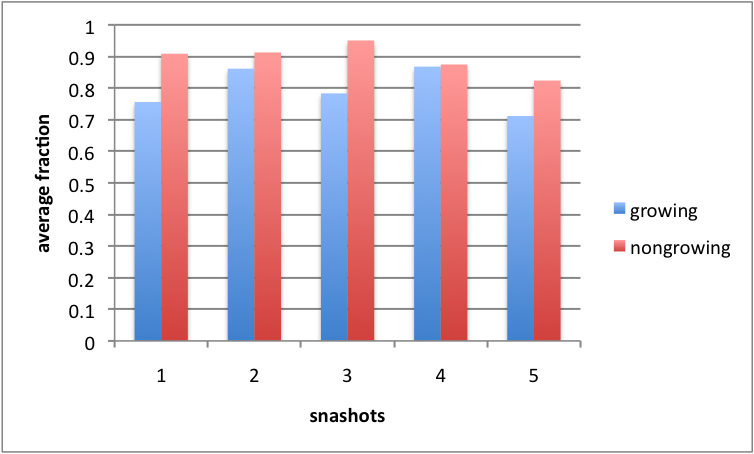
\includegraphics[width=80mm]{../figures/nonatt_growth.png}\caption{Percentage of unattractive members of growing and non-growing communities.}\label{fig: perc_unatt}
%\end{center}
%\end{figure}
